% $Id$
%

\documentclass[10pt]{article}
\usepackage{mathptmx}
\usepackage{courier}
\usepackage[T1]{fontenc}
\usepackage{textcomp}

\usepackage{epsfig}
\usepackage{listings}

\lstdefinelanguage{MYLANG}
{morekeywords={},
sensitive=false
}

% See the dvips documentation
% Shrink figures larger than the text width to the text width
\def\epsfsize#1#2{\ifdim#1>\columnwidth\columnwidth\else#1\fi}
%\def\epsfsize#1#2{\textwidth}
\epsfverbosetrue

\title{A Software Development Metaphor for Developing Semi-dynamic Web Sites through Declarative Specifications}

\author{Diomidis Spinellis, Vassilios Karakoidas and Damianos Chatziantoniou\\
Department Management Science and Technology\\
Athens University of Economics and Business\\
Greece\\
email: \{dds, bkarak, damianos\}@aueb.gr}

\date{}

\begin{document}

\maketitle

\begin{abstract}
\noindent
Traditionally, the realization of Web sites involves either
static content developed using web authoring tools or dynamic
content delivered by a database driven front-end,
where the structured content is organized
in a relational schema and dynamically generated on the fly.
The limitations of statically-authored web pages are easy to discern and
for a number of applications, the use of a database
introduces a level of additional complexity that
makes the choice a part of the problem space rather than the solution space.
Based on the distributed software development approach, we present a suitable for managing 
middle-sized semi-dynamic web sites. The technological dimensions of this
approach are well-known open source technologies, such as version control systems
and {\sc xml} transformation tools.
\end{abstract}

\subsection*{Keywords}
Web site development, semi-dynamic web sites, {\sc xml}, make, {\sc BibTeX}, {\sc xslt}, {\sc X-Schema (xsd)}, {\sc html}.

\section{Introduction}
\label{sec:intro}
Traditionally, the realization of Web sites involves either
static content developed using web authoring tools like
Microsoft's Front Page and DreamWeaver, or dynamic
content delivered by a data-oriented front-end,
where the structured content is stored in a relational database 
and dynamically generated on the fly.
When our group faced a series of problems with both the above approaches,
we decided to explore ideas for a radically different
implementation style, based on the declarative specification
of all the site's elements.

The limitations of statically-authored web pages are easy to discern.
The content is authored in an unorganized manner, and, as a result,
can be inconsistent in both structure and presentation.
While the use of cascading style sheets can help one obtain a
consistent look, their use still requires discipline.
Moreover, the authored pages remain unstructured and the resulting
site can be difficult to modify and reorganize.
Furthermore, the static authoring model often imposes a centralized
management and maintenance style;
all additions and changes have to go through a single person,
creating a bottleneck, often leading to outdated content.

Adopting a database driven approach is supposed to
solve the aforementioned problems.
Separating the source data from its (dynamically generated)
marked-up version ({\sc html} code) leads to a consistent
yet flexible generation of web pages.
In addition, the database's relational model imposes
its structure on the data being stored.
Finally, a database back-end allows concurrent updates by
different users.

However, for a number of applications, the use of a database
introduces a level of additional complexity that
makes the choice a part of
the problem space rather than the solution space.
A database-driven web site requires the implementation of a
front-side interface to transform the web site's content into
{\sc html} code, and a back-end interface to allow stakeholders
enter, review, and update data.
The back-end client interface typically requires setting up
and maintaining appropriate access permissions.
These may need to be integrated into an organization wide authentication 
facility, or operated under a specific security policy.
In the second case, procedures for setting up passwords,
resetting them, and revoking them need to be established and followed.
A properly running database also requires a skilled database
administrator to install it, maintain it, organize backups,
and perform modifications to the database schema.
In addition, marked-up content is generated by a front-end
program accessing the database, therefore the front-end and the database
must be extremely secure and robust \cite{VG01}, running on a $24 \times 7$ basis.
The front-end, being an executable program working on
untrusted data (the web page requests) can become the target of
malicious attacks,
and must therefore be inspected and audited to ensure its robustness \cite{YHDM04}.

To minimize the risk of an attack against the database
(that would jeopardize the organization's data)
the database server has to be installed on a machine separate
from the web server, behind a properly configured firewall.
Finally, the extraction of content from a database often
induces the web site's designers and stakeholders to adopt a
query-style interface.
Such an interface is typically less usable than browsable web pages,
and the served content is often ignored by search engines,
leading to reduced visibility
of the (meticulously structured) content \cite{DEEP_WEB, JP04}.

All in all, a database-driven approach appears to be suitable
only for those with ample resources to justify the full
development and appropriate maintenance of a sophisticated infrastructure.

Having faced the problems we described above within our organization,
we reasoned that a fresh approach was needed to tackle them.
Specifically,
in an internal effort to develop and maintain our group's web site
we had already abandoned the ad-hoc authoring tool--based approach
because it led to an inconsistent look and stale content,
while the maintenance of a subsequent database-driven
design approach was proving intractable for the resources that
our group could afford.
In the following sections we describe the methodology we developed
for implementing semi-dynamic web sites,
illustrate it by means
of a case study covering the requirements, design, and implementation,
and discuss the lessons we learned.

\section{Related Work}
\label{sec:related}

During the last decade, the World Wide Web became a popular platform for many {\sc IT} applications.
Researchers and companies, in their attempt to make robust and easily maintainable web applications,
developed many frameworks and tools to formalize and make efficient the creation and maintenance process.

Fraternali \cite{FRA99} analyzed and studied the perspectives of
web development. He pointed out, that the development process has
five distinct perspectives: (1) {\em process}, (2) {\em models, languages and notation}, (3) {\em reuse}, (4) {\em architecture} and (5) {\em usability}.
These include elements like {\em requirements}, {\em  prototyping and validation}, {\em evolution and maintenance}, that apply in
software engineering scientific areas, and other aesthetic elements like {\em visual quality} and {\em degree of proactivity}.
As we will see in section \ref{sec:req}, in our work we took into consideration all the above perspectives and we introduced a few more, like {\em openness}
and {\em observability}.
As a plus, in our methodology we implement the system taking into account the organizational aspect of maintainability of content and the underlying application.

In addition, Fraternali categorizes relevant software tools into six individual categories: (1) {\em visual editors and site managers},
 (2) {\em web-enabled hypermedia authoring tools}, (3) {\em web-DBPL (database programming languages) integrators}, (4) {\em web form editors, report writers,
 and database publishing wizards},
 (5) {\em multiparadigm tools} and (6) {\em model-driven application generators} \cite{FRA99}. These tools are both commercial and open-source and they are widely used.
 In section \ref{subsec:key-tech}, we will see that in our case we chose open source tools to satisfy the {\em openness} functional requirement.
 
Many research groups also designed and implemented frameworks to organize the web development process. These frameworks addressed issues
such as {\em lifecycle coverage}, {\em process automation}, {\em modeling abstractions}, {\em reuse and components}. The most popular implementations are 
Araneus \cite{MAM03}, 
Autoweb \cite{FP00} and Strudel \cite{FFLS00}. Many are extended to enhance their abilities. For example, the Strudel
framework introduced a declarative query language, called StruQL that was later extended by FunStruQL \cite{FST99}. Another interesting
framework is WebJinn \cite{KL03}. This framework tries to resolve the crosscutting concerns in web development.

All the above architectures are introducing development methodologies and languages/scriptlets to achieve their goals. For example, Strudel with StruQL
and Araneus with homer. Our goal was to create a system
that would depend only well-known technologies like {\sc xml} and {\sc cvs}.

For a successful high-level design of a web application, a visual notation also introduced to specify composition and navigation features in
hypertext applications. This language is {\sc WebML} \cite{CFB00,WEBML}, a language based on standards like Entity-Relationship model {\sc (erd)} and {\sc uml} \cite{UML}.
{\sc WebML} has been proposed in the context of {\sc W3I3} Esprit project.
Araneus also defined a logical model known as the Araneus Logical Model \cite{MAM03}.
These higher level abstractions are well defined and very useful for the overall design of a web site, but are based on custom technologies.
In our case we based our semantics on {\sc xml} and {\sc BibTeX} to provide a common data abstraction layer.

\section{Methodology}
\label{sec:meth}
Our proposed methodology for developing semi-dynamic web sites uses as
its metaphor the distributed software development activity, as popularized
by many high-visibility distributed open-source development projects,
such as Eclipse \cite{GB04}, Mozilla, and Free {\sc bsd}.
Using a metaphor as a guiding principle for a development activity
is a practice we adopted from extreme programming \cite{Bec00}.
The methodology can be summarized in a few key points.

\begin{itemize}
\item Structure the site's data as {\sc xml} files,
or another declarative formalism.
Content developers create and edit these to modify the site's contents.
\item Use {\sc xml} schemas and corresponding tools to validate the content.
\item Exploit modular {\sc xhtml} \cite{W3C_MODULAR_XHTML} to create schemas for rich
data elements.
These can be used to allow the inclusion of specific {\sc xhtml} tags
in the site's {\sc xml} files, without having to reinvent {\sc html}
from scratch.
\item Adopt a version control system for distributing the content,
templates, transformation, and schemas across content developers and
administrators, synchronizing updates, and keeping a record of the project's history.
(Thomas and Hunt \cite{HT00} aptly compare a version control system
with a global undo command with unlimited undo levels.)
\item Create the site's look and feel in {\sc xhtml} format
through {\sc xslt}  transformations \cite{HM01}.
\item Express verification and building dependencies among
data elements and schemas through {\em make} \cite{MAKE} or {\em ant}
\cite{JAKARTA_ANT} rules.
\item Make the local generation of the site's content the default
building option to allow developers and administrators to verify
the results of  their work, before putting them online.
\item Use existing mechanisms and tools, such as the secure session shell,
public key authentication, and group membership permissions to implement
authentication and authorization policies.
\item Have an instance of the project on a centralized server, kept up to
date through the version control system, as the source to generate and export
the definitive version web site's contents.
\end{itemize}

One can easily discern from the above points the similarities of our
approach with distributed software development.
A version control system is used to distribute the artefacts among
developers in their current form, and a building tool, such as {\em make}
or {\em ant} guides the building process.
Developers edit and build their work locally, and commit it to a central server when ready.
The repository on the central server is the source for creating the end-result
of the product, through a {\em daily build} process.
In our case however, the developers work with {\sc xml} and {\sc xslt}
files, instead of programming language source code files.

To illustrate our methodology in concrete terms
the following sections contain as a case-study the design and implementation
of our research group's web site.
Through the case study we will demonstrate the key points applied in
practice, discuss important technical and human issues we faced,
and present the lessons we learned.

\section{Requirements}
\label{sec:req}

\begin{figure}
\begin{center}
\leavevmode
\epsfbox{Diag.eps}
\end{center}
\caption{
\label{fig:diag}
Overview of data element relationships.}
\end{figure}

The functional requirements for our center's web site were
simple, but not trivial, and had already been satisfied
twice in two different forms.
The site should present our research center's members, groups, publications,
and projects in an organized fashion.
Our center is divided into five groups.
It numbers about 50 members, is a participant of 35 past and current research
projects, and the originator of about 400 publications.
The site's pages should represent the content and the relationships
we illustrate in Figure \ref{fig:diag}.
The self-referential relationship on the group entity exists because the center should  an ``umbrella'' group of multiple subgroups.
Members of our center and our research projects are associated
with one or more groups.
Publications are associated
with one or more members, groups and projects.
For the sake of simplicity,
we have omitted from our description and the diagram
a number of additional relationships,
such as the member directing a group or managing a project.
As an example of the type of content we were looking for, 
each member, group, or project should have a web page with a list
of the corresponding publications;
each group should have pages listing its projects and members. 
In order to have the ability add web site data that is not part of the aforementioned categories,
each group can have additional pages of unstructured {\sc xhtml} content, in a dictated manner.
Finally, each member of our groups may be performing a presentation in our group's weekly seminar.

As we hinted in the previous section, the problem with
the previous implementations was not the creation of the site
satisfying the functional specifications,
but the lack of a number of important non-functional requirements.
Before embarking on our third attempt,
we articulated those non-functional requirements
we thought important, to ensure that our third attempt would produce
a result with a longer life span.
The following is a list of the non-functional properties
we deemed important enough to guide our design.

\begin{description}
\item[Openness] The tools used in the realization of the web site
should be available as open source, or supported by multiple vendors.
We wanted to avoid becoming tied with a particular proprietary
tool.
We reasoned that openness would mitigate two risks:
(1) finding a maintainer trained to use a particular proprietary tool,
and (2) obtaining resources for upgrading and maintaining the tool.

\item[Observability]
The semantic distance between
the specification of an element and its implementation 
should be minimal \cite{SG97}.
The site's look and content should be maintainable
using standard tools and techniques.
If possible, the site's maintainer should not be required to
learn a scripting language like {\sc php}, or {\sc perl}, or
a framework like {\sc j2ee} or {\sc .net}.
An approach based on declarative specifications \cite{FFLS00} and
domain-specific languages \cite{DKV00, Spi00b} would allow end-users, or members
close to end-users to be involved in maintaining the site,
without risking the bottleneck of going through
multiple intermediaries.

\item[Robustness] The web site should not depend on
any external programs other than the web server for serving
its content.
Users updating the data, should be able to author, validate and 
review their changes without requiring network connectivity.
This would allow them to work productively over dial-up connections
or while on the road. In addition, all the editing users should be able 
to work on a platform of their choice ({\sc unix}, {\sc microsoft windows} and {\sc macintosh}) 
using only a text editor of their choice.
Minimizing the dependencies on additional servers (such as a
database or an application server) and on the network
should result in a more robust and easier to maintain system.   

\item[Parsimony] The implementation effort for
the system should be minimal.
This would minimize errors and maintenance costs.
We reasoned we could satisfy this requirement by
using existing tools, if their choice satisfied the
other non-functional properties.
\end{description} 

\section{Design Process}

\subsection{Conceptual Framework}

The system's conceptual framework is illustrated in Figure \ref{fig:conc-model}.
The main concept in our system is the {\em Organization}. Each {\em Organization} has 
information that interests {\em Content Consumers}. They 
access the organization's {\em Public Data}.
To obtain information regarding the {\em Organization}.
It has also {\em Content Developers} 
who are usually its members. {\em Content Developers} update the 
{\em Public Data} for the {\em Organization}. {\em Content Administrators} 
are supporting the {\em Content Developers} 
(mostly troubleshooting and account management)
and inspecting the submitted {\em Public Data}.

\begin{figure}[h!]
\begin{center}
\includegraphics[scale=0.6]{conc-model}
\end{center}
\caption{Conceptual design of our system}
\label{fig:conc-model}
\end{figure}

\subsection{Motivation and Design Paradigm}

Our main guiding principle was to create a continuous, multi-person 
development activity.
Live web sites continuously evolve;
adopting the content authoring paradigm implied
by our first approach was a mistake.
Empirical evidence supports this observation.
Figure \ref{fig:rankyear} illustrates the changes
in usability rankings given to 21 Greek government department
web sites between the years 2002 and 2003 \cite{G03}.
The X shape in the rank changes between the one year and the next
is, we believe, the result of statically authored web pages
degrading to a point of irrelevance, and then being overhauled
from scratch. The change of ranking can be explained as decay of the web site when dropping,
and re-engineering when rising.

A database-driven approach also hinders evolution.
Changes to the content's presentation require the modification
and installation of the front end page generator;
not a typical lightweight operation.
Changes to the data schema are even more intrusive
requiring a synchronized modification of the data,
the front end, and the back end.

\label{sec:design}
\begin{figure}[h!]
\begin{center}
\leavevmode
\def\epsfsize#1#2{\epsfxsize}
\epsfysize.8\vsize
\epsfbox{rankyear.eps}
\end{center}
\caption{Yearly changes in web site rankings}
\label{fig:rankyear}
\end{figure}

Continuous multi-person based projects are quite
common in software development.
Numerous programmers and engineers contribute and coordinate their work
through a version control system, like {\sc cvs} \cite{BF01} that
maintains a master repository of the source code.
Concepts like the \textit{daily build} \cite{CS95b} or the
\textit{current} and \textit{stable} branches, as practiced by
numerous open source projects, allow the maintenance
of a known-good product.
What we needed for our approach were appropriate,
declarative language-based formalisms for expressing our data,
its transformation into web pages, and an efficient
generation process.

\subsection{Processes}

\begin{figure}[h!]
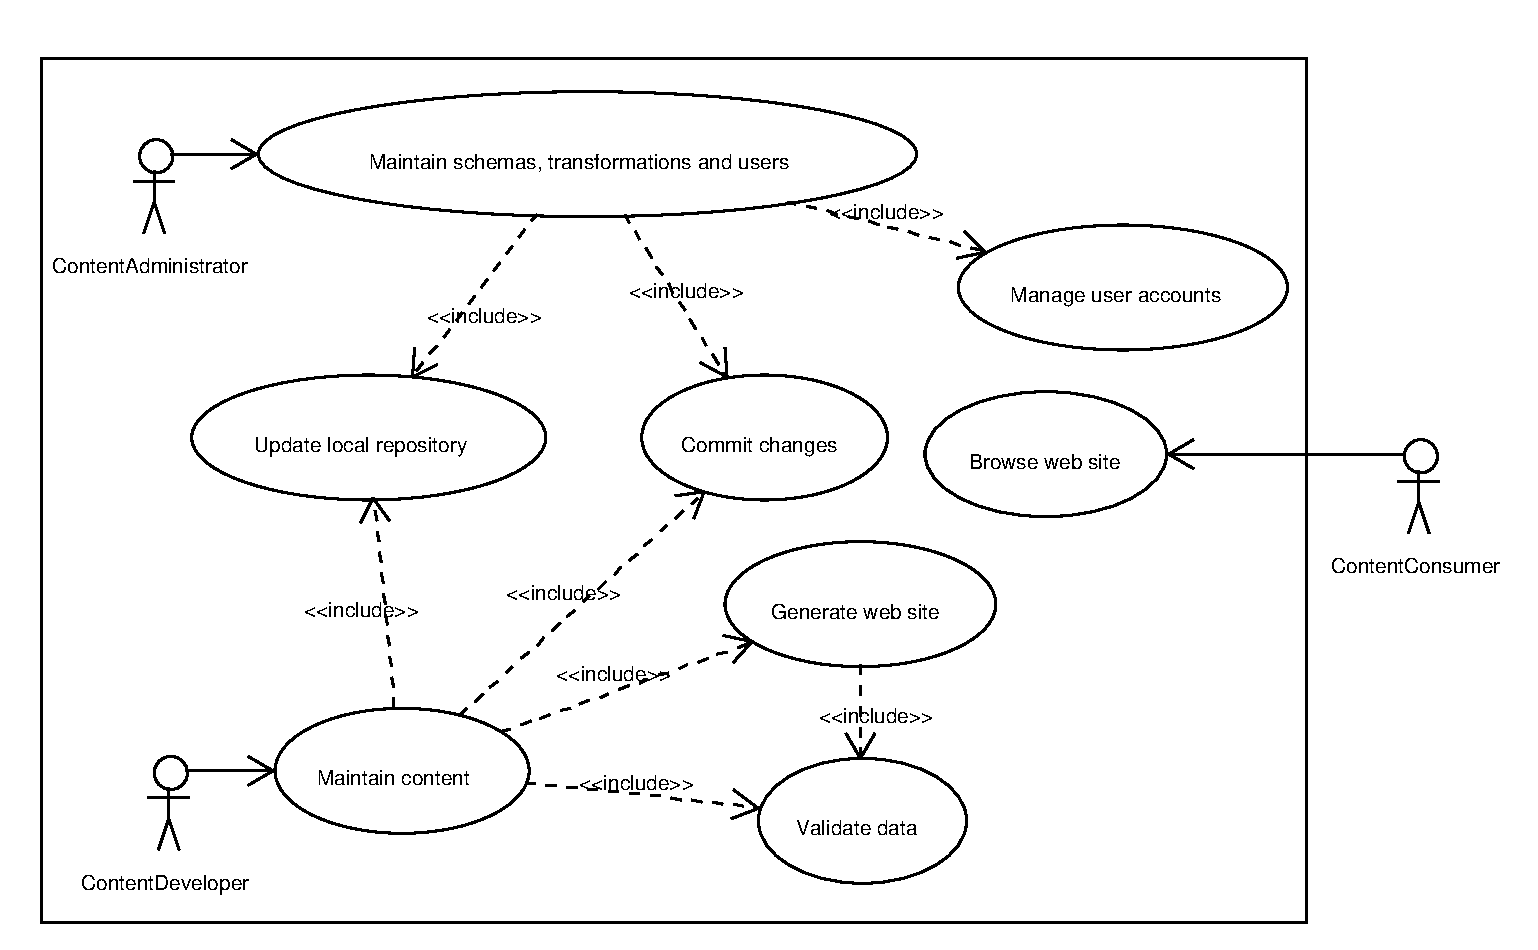
\includegraphics[scale=0.5]{use-case-diagram}
\caption{UML Use Case Diagram of the System}
\label{fig:use-case-diagram}
\end{figure}

Figure \ref{fig:use-case-diagram} shows a {\sc UML} \cite{UML} use case diagram of our system. 
We have three actors (roles) interacting with the system:

\begin{description}
\item[ContentDeveloper] A Content Developer is responsible for uploading data in the system. 
In our case, is typically a person for each research group. Content Developers can upload data files and 
import new bibliography entries.

\item[ContentAdministrator] The Content Administrator is responsible for the maintenance 
and the further extension of the system. A Content Administrator corrects problems with the data, develops 
new features or corrects existing ones in the transformation scripts.

\item[ContentConsumer] The content consumers are typically outside of our system
and have access only in the generated web site.
\end{description}

The use cases that comprise our system are:

\begin{figure}
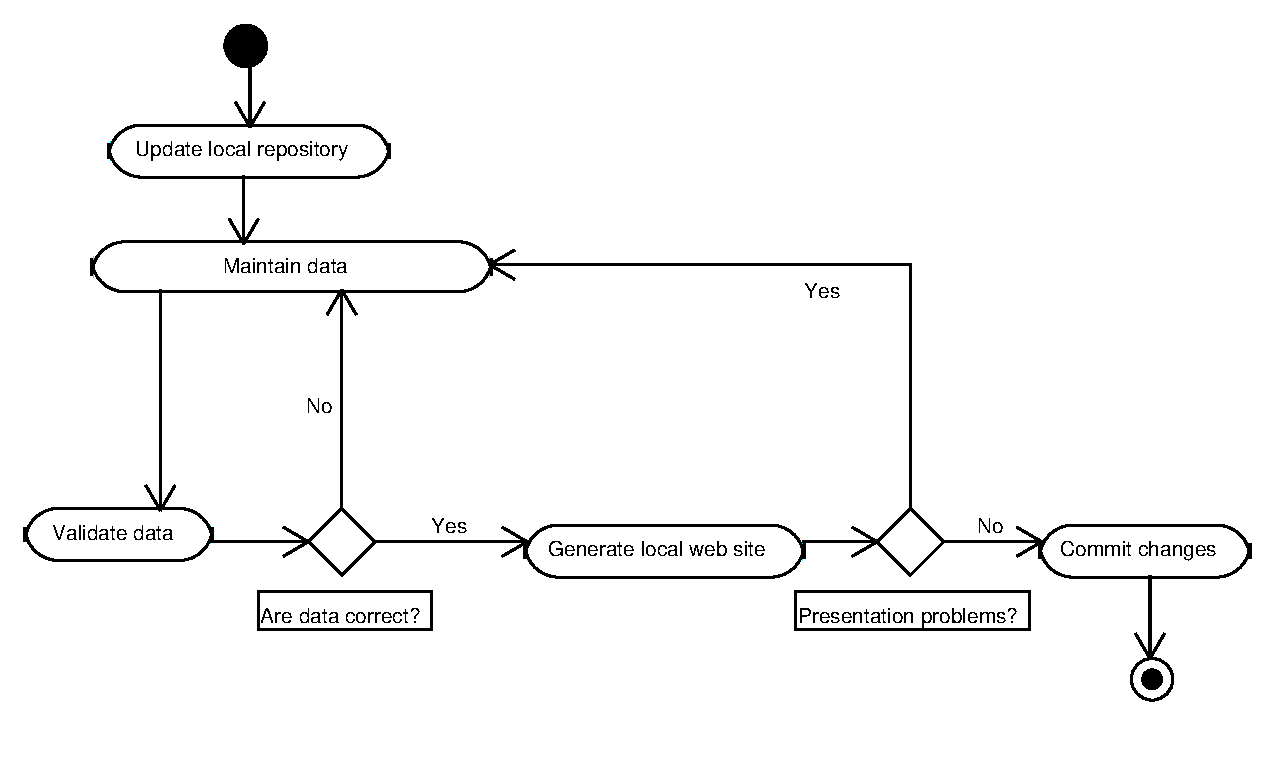
\includegraphics[scale=0.6]{maintain-content-activity}
\caption{UML activity diagram for Maintain Content}
\label{fig:maintain-content-diagram}
\end{figure}

\begin{description}
\item[Maintain schemas, transformations and users] This use case describes the 
maintenance and development procedures of the system. Each Content Developer can
update the data schemas the transformation scripts in order to correct errors 
and add new features.

\item[Update local repository] Content Developers have a local copy of the system's files on their workstation. 
and must update the local repository each time they use the system, in order to synchronize their local copy of the system with the master copy. 
To do so, they must execute an update 
repository command. If there is a conflict, the users must correct the problem 
and rerun the update command.

\item[Commit changes] Content developers and Content Administrators must commit 
the changes from their local repository to the {\sc cvs} repository in the web site server.

\item[Maintain content] This use case allows Content 
Developers to maintain the content of the web site. 
Content consists of group, member, project and seminar data or bibliography 
collection entries.

\item[Generate web site] Content administrators and developers can generate the 
web site locally for preview. Once the content is generated, 
the user can review the newly integrated content and inspect it
for possible presentation problems.

\item[Validate data] Content developers can validate the data in the local 
repository before the final commit. For the validation process
they use appropriate data schemas.

\item[Manage user accounts] Content Administrators perform user management in the 
system. User management consists of two main processes: 
(1) Authentication , (2) Ownership \& Policy.

\item[Browse web site] This one describes the web site browsing process.

\end{description} 

In Figure \ref{fig:maintain-content-diagram} we show the activity diagram of the 
most complex use case in the system. The Content Developer first updates the 
local repository and then begins data maintenance by adding, 
removing or modifying data files and bibliography entries. Upon completion, data 
validation must be performed before the commit to the data repository. If the data 
repository is valid, then local web site generation must be performed to validate the 
presentation. After that, the data is ready to be submitted to the main 
data repository. After the update of the data repository the process terminates.

\section{Implementation}

\subsection{Key Technologies}
\label{subsec:key-tech}

Once the design was finalized,
implementation proved to be an almost hollow activity,
since it did not involve almost anything of what
is typically described as coding.

The first step involved selecting and setting up the
appropriate tools. In order to meet the requirements we set in section \ref{sec:req}, 
we decided to use popular open
technologies as key elements of our system.
We adopted the concurrent versions system
({\sc cvs}) \cite{BF01, CVS} to coordinate the distribution
and update of all the system's components.
Authentication for managing content was handled by the
Unix group membership mechanism of the host where the
{\sc cvs} repository was installed.
We also used
{\sc BibTeX} \cite{Pa88, Lam94} and {\sc bib2xhtml} \cite{BibXHMTL} for transforming the publications
into {\sc xhtml} and
xmlstarlet \cite{Gru04} for validating and transforming
all other {\sc xml}-based data \cite{W3C_XML}.
For data transformations we 
implemented a system based on {\sc xslt} \cite{W3C_XSLT}, a language for transforming {\sc xml} documents.
Finally, {\sc gnu} {\em make} \cite{gnu_make} and a couple of shell script
constructs were used for handling the project's makefile.
The complete setup including all tools proved to be portable
between {\sc unix} and {\sc microsoft windows}, with team members working
on machines running different versions of {\sc microsoft windows}, {\sc gnu/linux},
and Free{\sc bsd}.

\subsection{System Development}

The next step was a series of iterations where we
modeled the data's schema on representative {\sc xml}
files. Concurrently, we implemented the validation {\sc dtd / xsd}s (Document Type Definition / X Schemas)
and the transformation {\sc xslt}s. First we developed the {\sc dtd}s
for the data validation, later on we decided to use {\sc xsd} schemas in order to perform
further data validation to our system.
The version control system was already proving its value
at this point
for coordinating the work between the two of the paper's authors.
Because many page elements, like a project's description,
could contain content more elaborate than plain text,
we used {\sc w3c}'s modular {\sc xhtml} specification for
importing existing elements in our {\sc dtd / xsd}s.
This helped us keep our schema description simple,
but the corresponding schema expressive.

\begin{figure}[h!]
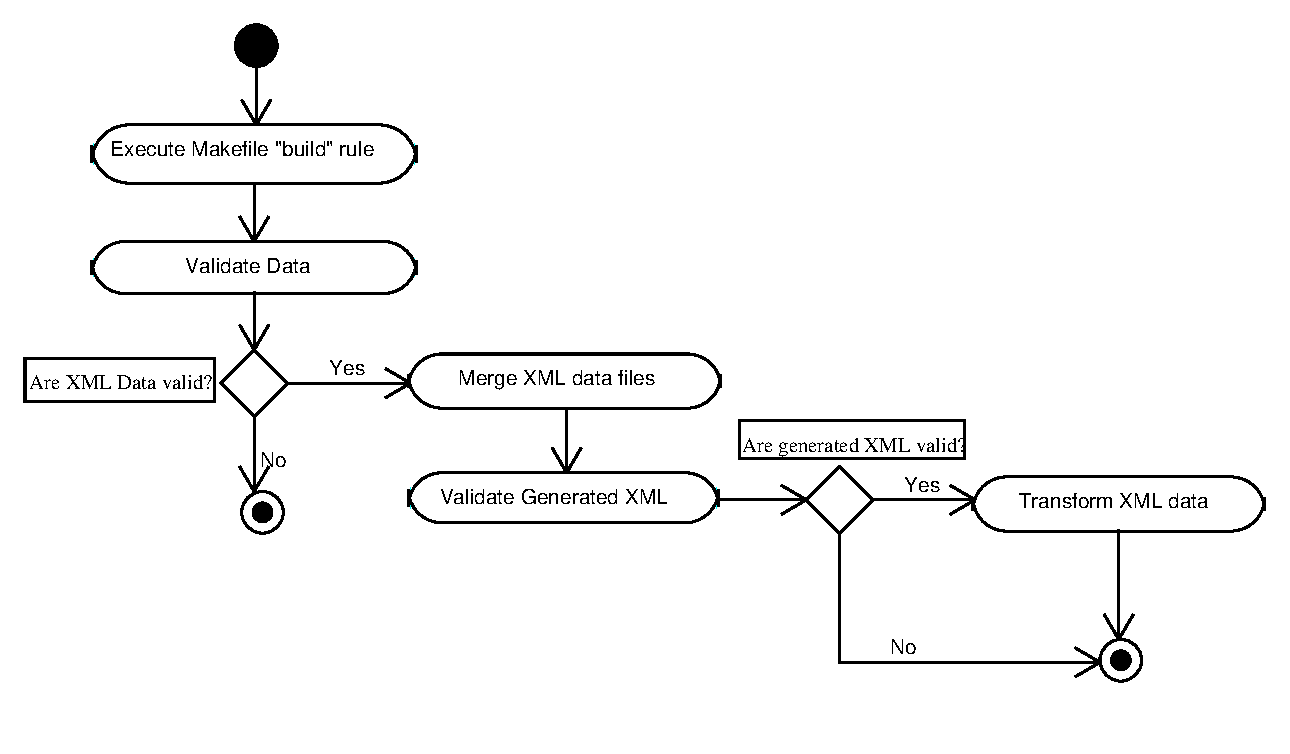
\includegraphics[scale=0.6]{generate-web-site}
\caption{UML Activity diagram for generating the web site}
\label{fig:generate-web-site}
\end{figure}

In Figure \ref{fig:generate-web-site} we illustrate the web site generation process.
The automated validation and generation of content was
expressed as makefile rules \cite{OTT91}.
The individual {\sc xml} files are merged in a
single {\sc xml} file for cross validating identifier
reference attributes ({\sc idref}s).
The same file is also used to extract the identifiers of
all projects, members, and groups into makefile
variables.
A simple loop then generates the {\sc xhtml} files
corresponding to each of the above elements.
Each project, member, group etc. refers to the relevant {\sc xml id}s.
Upon generation, links are created to
connect relevant generated pages e.g. each member hyperlinked with the corresponding publications, 
which are two different independently generated {\sc xhtml} pages.

The {\sc xhtml} content is, by default, generated on the
local machine, where its maintainer can verify it.
After the new content is validated and verified,
the maintainer can commit the change to the central {\sc cvs} repository. 
A separate makefile rule can then be used,
to execute an update command on the
host serving the content to the web.
The command retrieves the updated data from the {\sc cvs}
repository and regenerates the pages on the web-server's
file area.
All components of our system are under version control,
all pages are automatically tagged with identifiers
denoting their source, helping the traceability of changes.
All exchanges between the developers' machines and the
{\sc cvs} and web host are performed using the secure
shell ({\sc ssh}) as the transport protocol guaranteeing the data's integrity
and confidentiality.

\begin{figure}
\lstset{language=MYLANG,basicstyle=\ttfamily}
{\begin{lstlisting}
<xs:schema xmlns:xs="http://www.w3.org/2001/XMLSchema">
 <xs:element name="seminar">
  <xs:complexType>
   <xs:sequence>
    <xs:element name="sem_date">
     <xs:simpleType>
      <xs:restriction base="xs:string">
       <xs:pattern value="[0-9]{8}" />
      </xs:restriction>
     </xs:simpleType>
    </xs:element>
    <xs:element name="sem_time" type="xs:string" />
    <xs:element name="sem_title" type="xs:string" />
    <xs:element name="sem_room" type="xs:string" />
    <xs:element name="sem_url" type="xs:string" minOccurs="0" />
    <xs:element name="sem_duration" type="xs:string" />
   </xs:sequence>
   <xs:attribute name="by" type="xs:string" />
  </xs:complexType>
 </xs:element>
</xs:schema>
\end{lstlisting}}
\caption{Seminars X-Schema file}
\label{fig:project-dtd}
\end{figure}

\begin{figure}
\lstset{language=MYLANG,basicstyle=\ttfamily}
{\begin{lstlisting}
<?xml version="1.0"?>
<seminar by="m_bkarak">
 <sem_date>20040314</sem_date>
 <sem_time>19:00</sem_time>
 <sem_title>Regular Expressions</sem_title>
 <sem_room>906</sem_room>
 <sem_url>http://www.eltrun.gr/seminar/presentations.ppt</sem_url>
 <sem_duration>3 hrs</sem_duration>
</seminar>
\end{lstlisting}}
\caption{A typical seminar XML file}
\label{fig:project-xml}
\end{figure}

\begin{figure}
\lstset{language=MYLANG,basicstyle=\ttfamily}
{\begin{lstlisting}
<xsl:template match="seminar" mode="full">
 <h3><xsl:value-of select="sem_title" /></h3>
  <xsl:element name="a">
  <xsl:attribute name="name">
   <xsl:value-of select="sem_date" />
  </xsl:attribute>
</xsl:element>
 Presenter: <xsl:apply-templates 
 	     select="/eltrun/member_list/member [@id=current()/@by]" 
	     mode="simple-ref" /><br />
 Date: <xsl:call-template name="date">
	<xsl:with-param name="date" select="sem_date" />
       </xsl:call-template> <br />
 Time: <xsl:value-of select="sem_time" /><br />
 Duration: <xsl:value-of select="sem_duration" /><br />
 Location: <xsl:value-of select="sem_room" /><br /><br />
 <xsl:element name="a">
  <xsl:attribute name="href">
   <xsl:value-of select="sem_url"/>
  </xsl:attribute>
  Download the presentation
 </xsl:element>
</xsl:template>
\end{lstlisting}}
\caption{The XSLT transformation file for seminars}
\label{fig:project-xslt}
\end{figure}

\begin{figure}
\lstset{language=MYLANG,basicstyle=\ttfamily}
{\begin{lstlisting}
<tbody valign="top">
<tr>
<td align="left" width="82%">
<h2>Eltrun Seminars</h2>
<a href="index.html#20040314">14 March 2004 - Regular Expressions</a>
<br><br><br>
<h3>Regular Expressions</h3>
<a name="20040314"></a>
Presenter: 
<a href="../members/m_bkarak.html">
Mr. Vassilios Karakoidas
</a><br />
Date: 14 March 2004<br />
Time: 19:00<br />
Duration: 3 hrs<br />
Location: 906<br><br />
<a href="http://www.eltrun.gr/seminar/presentations.ppt">
Download the presentation
</a>
\end{lstlisting}}
\caption{A generated HTML seminar file}
\label{fig:project-html}
\end{figure}

You can see representative samples of a seminar's
{\sc xsd} schema description in Figure \ref{fig:project-dtd},
{\sc xml} data in Figure \ref{fig:project-xml},
{\sc xslt} transformation in Figure \ref{fig:project-xslt},
and {\sc xhtml} result in Figure \ref{fig:project-html}.

\begin{figure}
\includegraphics[scale=0.8]{distro.eps}
\caption{Directory structure of local repository}
\label{fig:eltrun-web-distro}
\end{figure}

The directory structure of a typical 
local repository is illustrated in Figure \ref{fig:eltrun-web-distro}.
Most of our users are working {\sc microsoft windows} environments and as 
a result we decided to upload a {\sc microsoft windows} version of the needed tools 
in the main repository under the directory \textit{bin}.
The directory \textit{data} contains the {\sc xml} and {\sc BibTeX} files and \textit{schema}
includes all the available {\sc dtd / xsd} and the modular {\sc xhtml} specifications.
The \textit{public\_html} and \textit{build} directory are used for the creation of the 
web site locally, while \textit{doc} contains the available documentation for the Content Developers
and Content Administrators. Finally, the directory \textit{tools} has a small selection 
of utilities ({\sc perl} and shell scripts) that provide statistical information
for our web site.

The installation procedure is very simple,
and the bootstrap tools it requires are only {\sc cvs} for 
the initial check out and an {\sc ssh} client. The needed keys 
for the secure shell session are provided once for each user by the Content Administrator. 
A full version of the system demands 8 megabytes of space 
on the local machine, plus some extra for the local content store and generation.

\begin{figure}
\includegraphics[scale=0.6]{dep-graph.eps}
\caption{Web graph of the generated site}
\label{fig:eltrun-web-m-dds-snapshot}
\end{figure}

In Figure \ref{fig:eltrun-web-m-dds-snapshot} we illustrate a web graph \cite{KRRSTU00} 
that shows references between the {\sc xhtml} pages.
The above Figure shows the references  of a member ("m\_dds" is the {\sc id} for 
Diomidis Spinellis), with other pages in the web site.
The pages starting with "p\_" are projects, with "m\_" members, and "g\_" groups.
At the time of writing the site generated 215 {\sc xhtml} pages with 2432 hyperlinks. 

\section{System Adoption}
\label{sec:adopt}

Our research center is multidisciplinary: under its roof
are both specialized software engineers using the same tools
we adopted in their everyday work, and researchers whose
background is management science, marketing, or finance
who are comfortable with {\sc gui} interfaces.
Upon completion of the development, we were somewhat concerned by the way our group
would receive the new way of work we proposed, in order to maintain the web content.

Our fears were justified.
The first presentation of the system to its users ended
almost in a revolt.
Non-technical users expressed their inability to comprehend
what an {\sc xml} document was, while technical members
helpfully argued for providing a {\sc gui} front end.
By targeting the users with the least technical experience,
promoting our system's ``soft'' attributes,
such as the use of open source software tools,
and convincing them to try to enter a few elements into
the system, we were able to overcome the initial reservations
and start the data migration process.

The next round of problems surfaced when users began entering
malformed or invalid data into the system.
This resulted in all users acquiring the copies of the malformed
{\sc xml} files, and strange error messages given to unsuspecting
users.
As is the custom in a number of development efforts, we had
expected the users to verify the changes they made before
committing them into the {\sc cvs} repository.
Non-technical users were however not aware of this etiquette
and were committing their changes with the hope they were correct.
A shared mailing list had established to explain the
importance of following the correct procedures when committing changes.
We also instituted a ``pointy hat'' policy. Committing a malformed file would award 
its committer a (virtual) ``pointy hat'', which would then be passed on to the next committer to err.
After a few days we got the impression that non-technical users
were becoming confident in their work, even proud of sharing
sophisticated tools and processes with software engineers.
Our technical persons experienced more problems than the inexperienced ones 
and that came as a surprise for us. Some of them were already familiar 
with the key technologies, and they tried to change the tools proposed with others 
more user-friendly. 
These initiatives resulted in corruption of the local repositories, malformed 
{\sc xml} data and wrong bibliography entries.
After a few false attempts they decided to stay with the procedures of the system.

Two weeks after the initial system presentation all users where able to upload 
and maintain their data. The inexperienced users learned how to edit {\sc xml} files,
importing {\sc BibTeX} entries into the system and committing to the {\sc cvs} repository. 
They just followed steps in a procedure that they see as a black box. 

\section{Lessons Learned}
\label{sec:concl}

We believe that our approach and many of the lessons we learned
can be applied in numerous similar situations,
leading to a lightweight, structured, consistent, and maintainable
web site building method. The proposed design satisfies the non-functional properties
we listed in Section \ref{sec:req},
and that our approach stands a higher chance to succeed where the
two other approaches failed.
The initial user reaction was not favorable, but this can
be explained by the significantly higher requirements we
placed on our users. Typical users are not well acquainted
with command line tools, and often see them as a threat to their productivity.
Instead of giving instructions by email to an unfortunate
web site maintainer, they now had to become active members
of an evolving web site maintenance effort.
Not all members of our research center proved ready to take
this responsibility.
Many groups delegated the maintenance to a single person. 
Others started with a centralized approach and later divided the
maintenance responsibilities as they came to appreciate the efficiency
benefits of the distributed site maintenance.
Still, however, we succeeded in distributing the previously
entirely centralized maintenance effort across our groups.
Summarizing, we believe that adopting a software development
metaphor and tools for developing and maintaining semi-dynamic
web site is a practical and worthwhile approach.

\begin{figure}[h!]
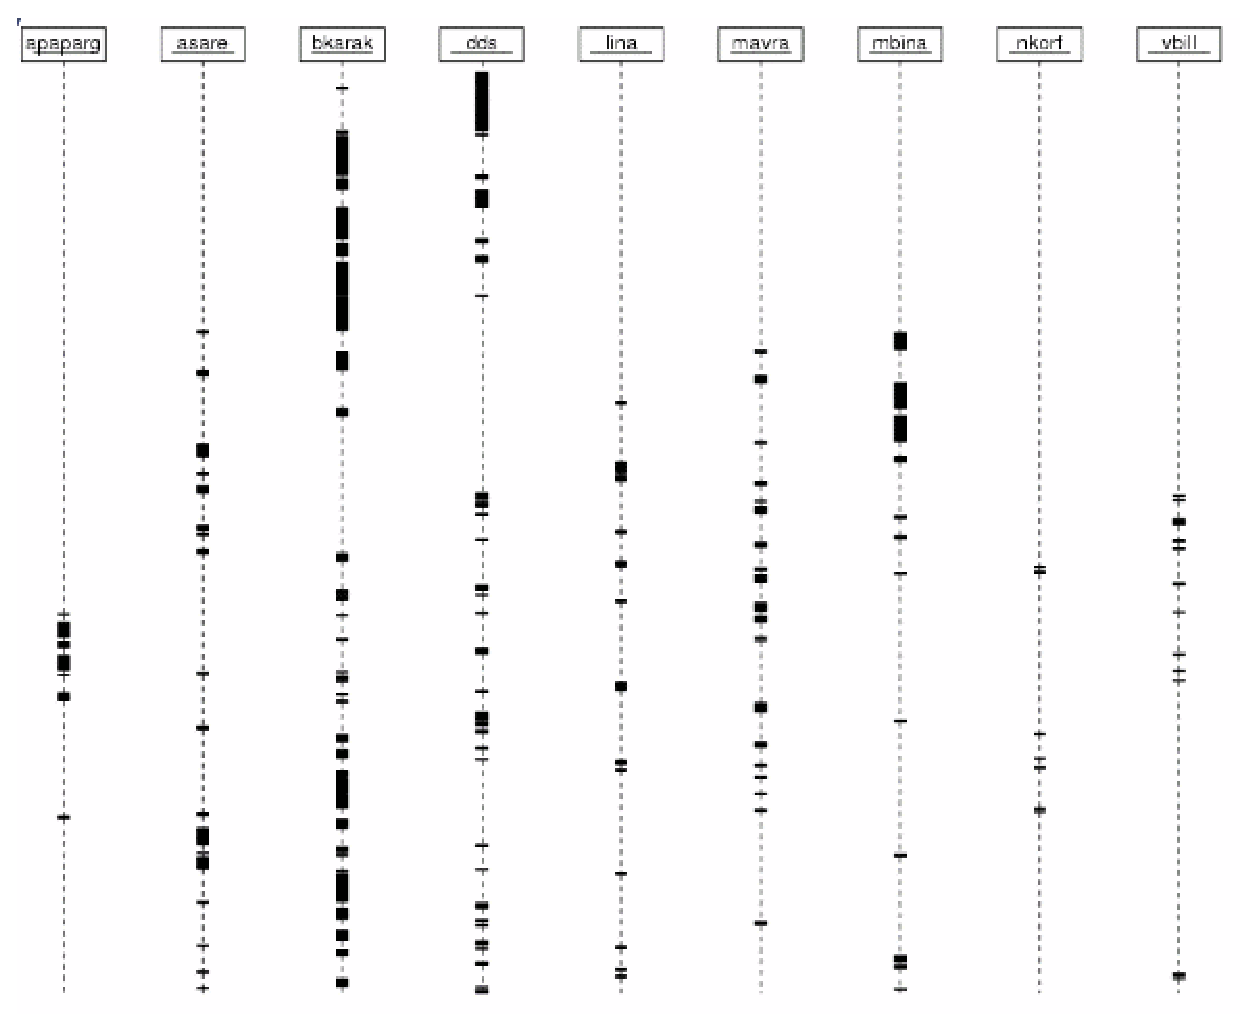
\includegraphics[scale=0.6]{cvs-log.eps}
\caption{Commit progress time line}
\label{fig:cvs-log}
\end{figure}

In Figure \ref{fig:cvs-log} we illustrate the {\sc cvs} \textit{commit} commands that have been performed by
the Content Developers and Administrators. Each swimlane in the Figure represents a committing
member of our system. Each horizontal tick represents a single commit instance.

Content Administrators are \textit{dds} (Diomidis Spinellis) and \textit{bkarak} (Vassilios Karakoidas). 
During the initial lit we can see that only the two committed 
changes. It was the development period of the system. After the initial development, a few 
pioneer content developers started to use the system and commit {\sc xml} and bibliography data. In this period 
we also tested the system thoroughly and developed the finalized the presentation of the web site. After the end of
the test period all users became active and began to commit data in a parallel manner. Figure \ref{fig:cvs-log} proves that we achieved 
one of our primary goals, converting the web site maintenance monolithic procedure into a distributed over time and multiple user development activity.

\section{Acknowledgments}
\label{sec:ack}

We would like to thank Prof. Manolis Skordalakis for his very perceptive comments during the compilation of this paper.
The authors would also like to thank George Oikonomou and Marianthi Theocharidou who reviewed versions 
of this paper and provided many corrections and observations.

\bibliographystyle{unsrt}
\bibliography{declweb}

\section*{Biographies}
\noindent
{\em Diomidis Spinellis} is an Associate Professor at the Department of Management Science and Technology at the Athens University of Economics and Business, 
Greece.  His research interests include software engineering tools, programming languages, and computer security.  He holds an MEng in Software Engineering 
and a PhD in Computer Science both from Imperial College (University of London, UK).  He has written more than 70  technical papers in the areas of 
software engineering, information security, and ubiquitous computing.  His book ``Code Reading: The Open Source Perspective'' 
received a ?Software Development Productivity Award? in 2004.  He has contributed software to the BSD Unix distribution, the X Window System, 
and is the author of a number of open-source software packages, libraries, and tools.

{\em Dr. Spinellis} is a member of the ACM, the IEEE, the Greek Computer Society, the Technical Chamber of Greece, and a founding member of the Greek 
Internet User's Society.  He is a co-recipient of the Usenix Association 1993 Lifetime Achievement Award.
\\
\\
{\em Vassilios Karakoidas} is a PhD candidate in Athens University of Economics and Business at the Department of Management Science and 
Technology. He holds an BSc in Computer Science (University of Piraeus) and an MSc in Information Systems (Athens University of 
Economics and Business). He is former member of the Health Informatics laboratory at University of Piraeus. He is now a member of 
ELTRUN/SENSE and has been involved in various research projects. The most recent are GEMINI and PRAXIS. His research interests include
Software Engineering, Programming Languages, Operating Systems and Networking.
\\
\\
{\em Dr Damianos Chatziantoniou} is visiting assistant professor in Athens University of Economics and Business and scientific consultant to 
ELTRUN. He has received his B.Sc. in Applied Mathematics from the University of Athens in Greece and continued his studies in Computer 
Science at New York University (M.Sc., 1993) and Columbia University (Ph.D., 1997), working with Ken Ross on data warehousing and decision
support systems. During his studies he was teaching and consulting regularly. Since 1997, Damianos is an assistant professor at Stevens 
Institute of Technology, an adjunct professor at Columbia University and president and co-founder of Panakea Software Inc. Panakea owns 
patent-pending algorithms for OLAP applications and developed a state-of-the-art decision support querying tool. Reference sites include AT-T, 
New York Hospital and Dun-Bradstreet. Damianos is collaborating with AT-T Labs-Research, Columbia University Medical Informatics Center, and 
National Technical University of Athens. His interests lie in the areas of data warehousing, decision support systems, OLAP and data mining. 
He has published papers and journals in VLDB, ICDE, EDBT and elsewhere.

\end{document}
